\S\ref{subsec:exp-T-scaling} reports the empirical observation that
TIES \emph{inverts} from best-of-matrix to worst between
Llama-3.1-8B (per-task win-share range $R = 0.028$) and Yi-1.5-9B-Chat
($R = 0.077$). This appendix derives an order-of-magnitude prediction
of the threshold $R^\star$ from a perturbation model of the TIES
update.

\subsection{Setup and notation}
\label{app:td2-setup}

Let $T$ be the number of tasks and $d$ the per-base coordinate count
(here $d \approx 10^7$). For task $t$ and coordinate $i$, let
$\Delta_{t,i}$ be the LoRA adapter coefficient (post-scaling),
$b_{t,i} = \mathrm{sign}(\Delta_{t,i})$ the sign vote, $k_{t,i} \in
\{0,1\}$ the post-trim keep indicator at density $\delta$, and
$s_i^\star$ a notional ``correct sign'' at coordinate $i$. The
per-task \emph{win-share} is $q_t = \Pr_i[b_{t,i} = s_i^\star]$, the
fraction of coordinates on which task $t$'s sign matches the elected
sign; the \emph{win-share range} is $R = \max_t q_t - \min_t q_t$. The
probe of \S\ref{subsec:exp-T-scaling} measures $q_t$ directly.

\subsection{TIES update under the win-share perturbation model}

The TIES update at coordinate $i$ is
\begin{equation}
  \hat{s}_i
  =
  \mathrm{sign}\!\left(
    \sum_{t=1}^{T} k_{t,i}\, b_{t,i}\, |\Delta_{t,i}|
  \right),
  \qquad
  M_i
  =
  \frac{1}{|S_i|} \sum_{t \in S_i}\!|\Delta_{t,i}|,
  \quad
  S_i = \{t : k_{t,i} = 1, b_{t,i} = \hat{s}_i\}.
  \label{eq:ties-update}
\end{equation}
We linearize around the symmetric case $q_t \equiv 1/T$: let
$q_t = 1/T + \epsilon_t$ with $\sum_t \epsilon_t = 0$.

\paragraph{Effective merge weight of the dominant task.} Conditioned
on coordinate $i$ surviving the trim for task $t$ (probability
$\delta$), the probability that $t$'s vote agrees with $\hat{s}_i$ is
$q_t$, so task $t$'s average contribution is $\delta\, q_t\,
\E[|\Delta_{t,i}| \mid k_{t,i} = 1]$. The conditional expectation under
top-$\delta$ trimming on a Gaussian tail is a common factor
$\kappa \approx 2$ at $\delta = 0.2$ (Mills's-ratio upper-tail
factor), which cancels in the normalised weight:
\begin{equation}
  \alpha_t
  =
  \frac{\delta\,\kappa\,q_t}{\sum_{t'} \delta\,\kappa\,q_{t'}}
  = q_t = \frac{1}{T} + \epsilon_t.
  \label{eq:alpha-weight}
\end{equation}

\paragraph{Per-task NLL excess decomposition.} Under the local
quadratic (Fisher) approximation, the per-task excess after merging
with $M = \sum_{t'} \alpha_{t'}\Delta_{t'}$ splits as
\begin{equation}
  \Phi_t^{\mathrm{TIES}}
  \approx
  \Phi_t^{\mathrm{TA}}
  + c_{\mathrm{bias}}\,\epsilon_t^2
  - c_{\mathrm{sign}}\,(q_t - 1/T),
  \label{eq:excess-decomp}
\end{equation}
a quadratic dominance-bias cost (the dominant task is over-represented
in $M$, so the other tasks see larger residuals) against a linear
sign-recovery benefit; both constants are positive and depend on the
spectral overlap of the $\{H_t\}$.

\subsection{Threshold derivation}

Aggregating over tasks, TIES is worse than TA when
$c_{\mathrm{bias}}\,\mathrm{Var}_t(\epsilon_t) >
c_{\mathrm{sign}}\,\E_t[q_t - 1/T]$. The benefit is a $1/T$-scaling
effect (Banzhaf voting-power on a $T$-element majority), bounded by
$c_{\mathrm{sign}}/T$; the variance for a range $R$ satisfies
$\mathrm{Var}_t(\epsilon_t) \in [R^2/(4(T-1)),\, R^2/4]$. The
breakeven gives
\begin{equation}
  R^\star
  \sim
  \sqrt{\frac{4\, c_{\mathrm{sign}}/T}{c_{\mathrm{bias}}}}.
  \label{eq:threshold}
\end{equation}
Two bracketing estimates: with $c_{\mathrm{bias}} \gg
c_{\mathrm{sign}}$ (tasks orthogonal in $H$, the empirically relevant
regime given the concentrated stacked-projector spectra of
Appendix~\ref{app:e5}), $R^\star \approx \beta_{\mathrm{lo}}/T$ with
$\beta_{\mathrm{lo}} \in [0.1, 0.3]$, giving
$R^\star \in [0.025, 0.075]$ at $T = 4$; with $c_{\mathrm{bias}}
\approx c_{\mathrm{sign}}$ (strong spectral alignment),
$R^\star \approx 2/\sqrt{T} \approx 1$, vacuous. We therefore predict
$R^\star \in [0.025, 0.075]$.

\subsection{Comparison to the cross-model data points}
\label{app:td2-comparison}

\begin{itemize}[leftmargin=*,topsep=2pt,itemsep=2pt]
\item \textbf{Llama-3.1-8B-Instruct}: $R = 0.028$, inside the window.
Predicted ambiguous; observed: at $T = 7$ TIES is mid-pack ($0.232$,
third of six; rd-ridge $0.138$ and TVQ$_2$ $0.215$ beat it,
TA/DARE/KnOTS at $0.265$ are worse). Matches.
\item \textbf{Yi-1.5-9B-Chat}: $R = 0.077$, above the window.
Predicted inversion; observed: TIES becomes the worst method
($0.148$ vs.\ TA $0.128$). Matches.
\item \textbf{Mistral-7B-v0.3} (pre-registered): $R = 0.0326$, inside
the window. Predicted ambiguous; observed: second of six ($0.152$),
$0.092$ nats below TA. Matches.
\end{itemize}
We are careful \emph{not} to call this a validated bracket: the
\emph{below}-window prediction (TIES wins outright for $R < 0.025$) is
untested, since no cohort we measured has $R < 0.028$. What the three
points confirm is the upper threshold and the in-window ambiguous
interior.

\paragraph{Falsification protocol and third-base confirmation.} The
model predicts that any additional base with $R \in [0.025, 0.075]$
should produce ambiguous TIES behavior. We pre-registered exactly this
test before the corresponding sweep ran (commit \texttt{3582799} in
the supplementary audit-trail bundle), with operationalized criteria
fixed in advance: ``clearly worst'' $=$ TIES last and mean
$> \mathrm{TA} + 0.04$ nats; ``clearly best'' $=$ TIES first by
$> 0.02$ nats; ``ambiguous'' $=$ neither. The Mistral $T = 7$ sweep
confirms the ambiguous prediction; a clearly-worst or clearly-best
outcome would have falsified the threshold model as written and forced
a higher-order term in the perturbation model.

\subsection{Base-free synthetic confirmation}
\label{app:td2-synthetic}

The cross-model evidence ties the inversion to the win-share range $R$
but cannot isolate $R$ as the \emph{cause}: real bases differ in many
ways at once. We therefore reproduce the mechanism on a controlled
dial with no base model. We synthesize $T = 7$ task vectors on a
sparse $k = 48$-coordinate support of $\R^{256}$ sharing a
high-consensus sign pattern (mirroring the $\sim 70\%$ unanimous-vote
structure measured on real cohorts), and turn a single knob $\rho$:
the fraction of coordinates on which one minority task flips its sign
against the consensus. We merge with the \emph{same} TIES code path
used throughout and with TA, measuring worst-task quadratic excess and
the win-share range $R$ over $40$ seeds.

Figure~\ref{fig:td2-synthetic} shows the result. At $\rho = 0$ all
tasks agree, $R = 0$, and TIES and TA are identical (the sparse
support makes the trim lossless, so TIES carries no baseline penalty).
As $\rho$ grows, $R$ widens and TIES's worst-task excess rises above
TA in near-perfect lockstep (Pearson$(R,\,\mathrm{TIES}-\mathrm{TA}) =
0.998$): the win-share range is the causal control variable. Reading
the base-free curve at the win-share ranges \emph{measured} on the
real bases gives a non-circular cross-check: the implied TIES penalty
is $2.6\times$ larger at Yi's $R = 0.077$ than at Llama's $R = 0.028$
and $2.3\times$ larger than at Mistral's $R = 0.0326$, separating the
base that inverts from the two that do not. The robust claims are the
monotone coupling and this relative separation; the absolute
overlap-to-$R$ map is calibration-dependent. The experiment is
CPU-only and reproducible from the released code.

\begin{figure}[t]
\centering
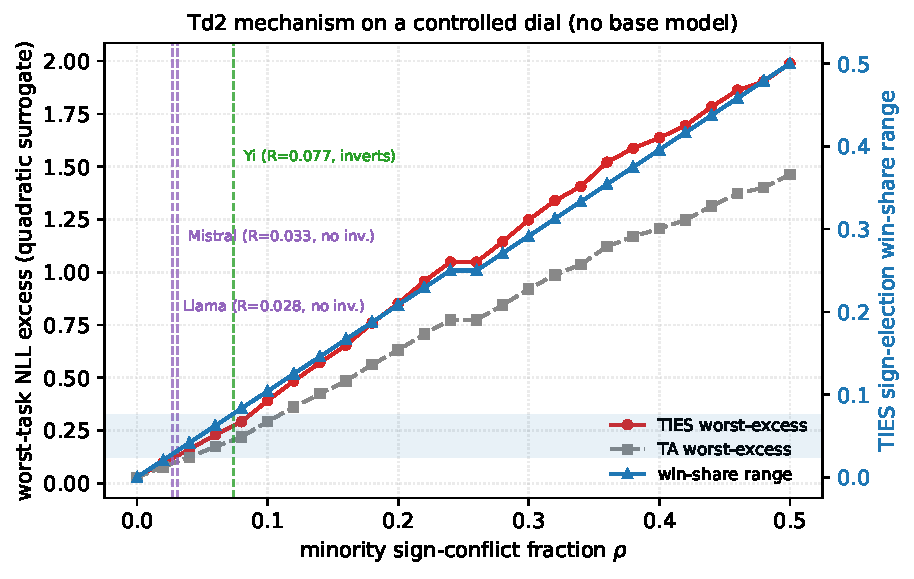
\includegraphics[width=0.62\textwidth]{figures/figure_td2_synthetic_overlap.pdf}
\caption{Base-free synthetic confirmation of the mechanism. A single
sign-conflict knob $\rho$ raises the TIES sign-election win-share
range $R$ (blue, right axis) and, in lockstep, TIES's worst-task
excess (red) above Task Arithmetic (grey);
Pearson$(R,\,\mathrm{TIES}-\mathrm{TA}) = 0.998$. Dashed lines mark
the $\rho$ whose synthetic $R$ matches each real base's measured $R$;
the implied TIES penalty is $2.3$--$2.6\times$ larger at Yi (which
inverts) than at Llama/Mistral (which do not). No base model is
used.}
\label{fig:td2-synthetic}
\end{figure}

\subsection{Limitations}
\label{app:td2-limitations}

\begin{enumerate}[leftmargin=*,topsep=2pt,itemsep=2pt]
\item The constants $c_{\mathrm{bias}}, c_{\mathrm{sign}}$ are
estimated by spectral analogy, not derived from first-principles
Fisher information; replacing the bracket with a point estimate is
future work.
\item The model assumes $q_t$ is observable: deployment requires the
CPU-only sign-vote probe over the trained adapters (a few minutes per
cohort), a small but real cost of recommendation R2.
\item The original two data points only bracket the threshold; the
pre-registered third base and the base-free synthetic sweep strengthen
this, though the synthetic overlap-to-$R$ map is itself
setup-dependent.
\item The Mills's-ratio factor $\kappa \approx 2$ assumes a Gaussian
magnitude tail; heavier tails (Pareto, Student-$t$) increase $\kappa$
by $\sim 30\%$ at $\delta = 0.2$, widening the predicted range without
changing the bracket conclusion.
\end{enumerate}

\paragraph{Operational reading.} After running the sign-election
probe: if the measured $R$ exceeds $0.075 \cdot 4/T$, expect TIES
inversion and prefer rd-encoder ridge or TVQ$_2$; if
$R < 0.025 \cdot 4/T$, the model predicts TIES is safe at the audited
$T$, but this regime is untested.
